\documentclass[10pt]{beamer}

\usetheme[progressbar=frametitle]{metropolis}
\usepackage{appendixnumberbeamer}
\usepackage{multicol}
\usepackage{booktabs}
\usepackage[scale=2]{ccicons}
\usepackage[style=authoryear]{biblatex}
\bibliography{demo.bib}
\usepackage{pgfplots}
\usepackage{bbm}


\usepgfplotslibrary{dateplot}


\usepackage{xspace}
\newcommand{\themename}{\textbf{\textsc{metropolis}}\xspace}

\title{Labor Markets and Technological Change: Evidence from Electronic Health Records}

\subtitle{Hanna Glenn}
 \date{\today}
% \date{}
%\author{Presented by: Hanna Glenn}
% \institute{Center for modern beamer themes}
% \titlegraphic{\hfill\includegraphics[height=1.5cm]{logo.pdf}}

\begin{document}

\maketitle

\setbeamercolor{background canvas}{bg=white}

\begin{frame}{Table of Contents}
  \setbeamertemplate{section in toc}[sections numbered]
  \tableofcontents%[hideallsubsections]
\end{frame}

\section[Motivation]{Motivation}

\begin{frame}{What is an EHR?}
\begin{itemize}
    \item Computer-program technology that hospitals purchase
    \vspace{3mm}
    \item What EHR is used for depends on level purchased:
    \vspace{2mm}
    \begin{itemize}
        \item All include electronic patient records
        \vspace{2mm}
        \item More complex systems allow for decision making assistance
        \vspace{2mm}
        \item More recently, patient interfaces are being developed
    \end{itemize}
\end{itemize}
\end{frame}

\begin{frame}[fragile]{HIT: Great (Expected) Potential in Healthcare}
\begin{alertblock}{Cost Saving}
\begin{itemize}
    \item Possible cost reduction of hundreds of billions of dollars \\ (\cite{hillestad2005})
\end{itemize}
\end{alertblock}

\begin{alertblock}{Quality Improvement}
\begin{itemize}
    \item Improved efficiency, patient safety improvements, physicians have decision support that could prevent unnecessary complications, etc.
    \item Significant policy push for EHR implementation: HITECH Act, 2008 provided financial incentive for hospitals to implement EHRs \nocite{hitech}
\end{itemize}
\end{alertblock}

\textcolor{blue}{The percentage of hospitals with basic EHR capability rose from 9$\%$ in 2008 to 84$\%$ in 2015.} (\cite{stats})

\end{frame}

\begin{frame}[fragile]{What does this mean for physicians?}
In the short run:
\begin{itemize}
    \item Physicians spend more time entering information into a computer and learning a new software
    \item Physicians have experienced significant burn-out from using and learning EHRs
\end{itemize}

In the long run:
\begin{itemize}
    \item Could make daily tasks easier or harder
    \item Continued loss of autonomy as technology progresses
\end{itemize}

\end{frame}

\begin{frame}[noframenumbering]{Physician Burnout in the Media}
\begin{center}
    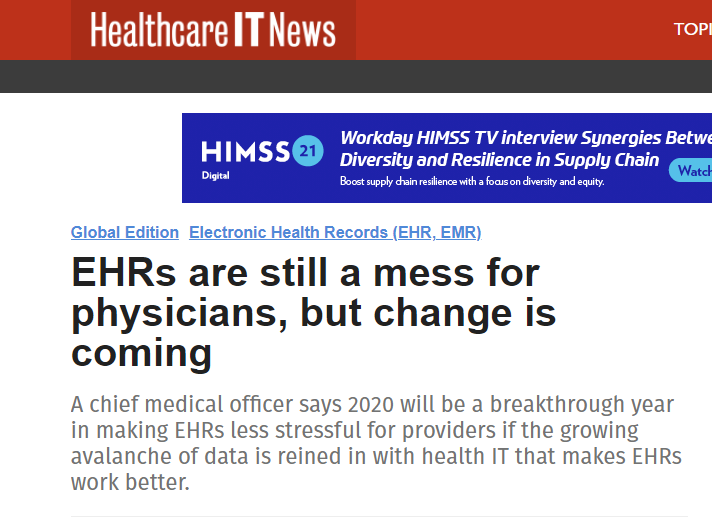
\includegraphics[scale=.4]{graphics/News Clip1.PNG}
\end{center}
\end{frame}

\begin{frame}[noframenumbering]{Physician Burnout in the Media}
\begin{center}
    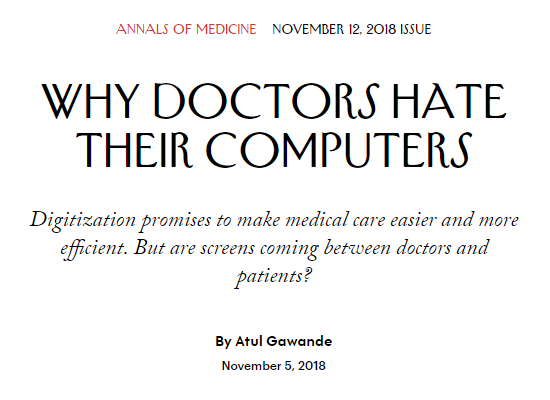
\includegraphics[scale=.5]{graphics/News Clip2.PNG}
\end{center}
\end{frame}

\begin{frame}[noframenumbering]{Physician Burnout in the Media}
\begin{center}
    
\includegraphics[scale=.45]{graphics/News Clip3.PNG}
\end{center}
\end{frame}

\begin{frame}{This Paper}

Did EHR implementation in hospitals affect labor market decisions of physicians, specifically where, and how much they work?
    
\end{frame}


\section{Contribution}

\begin{frame}{Branches of Literature}
\centering
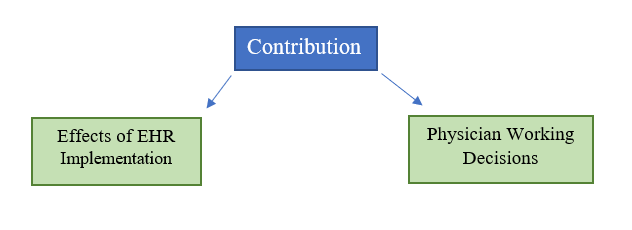
\includegraphics[scale=.5]{graphics/Contribution_litgraphic.PNG}

\end{frame}

\begin{frame}{Physician Labor Literature}
\centering
    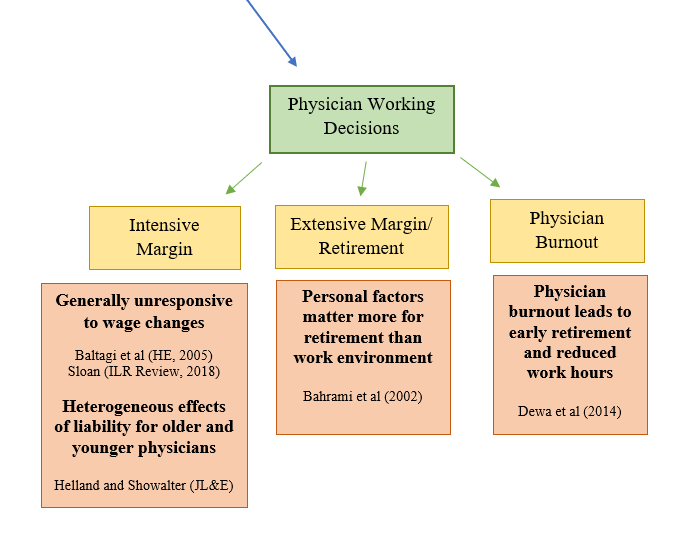
\includegraphics[scale=.45]{graphics/labor_litgraphic.PNG}
\end{frame}

\begin{frame}{EHR Literature}
    \centering
    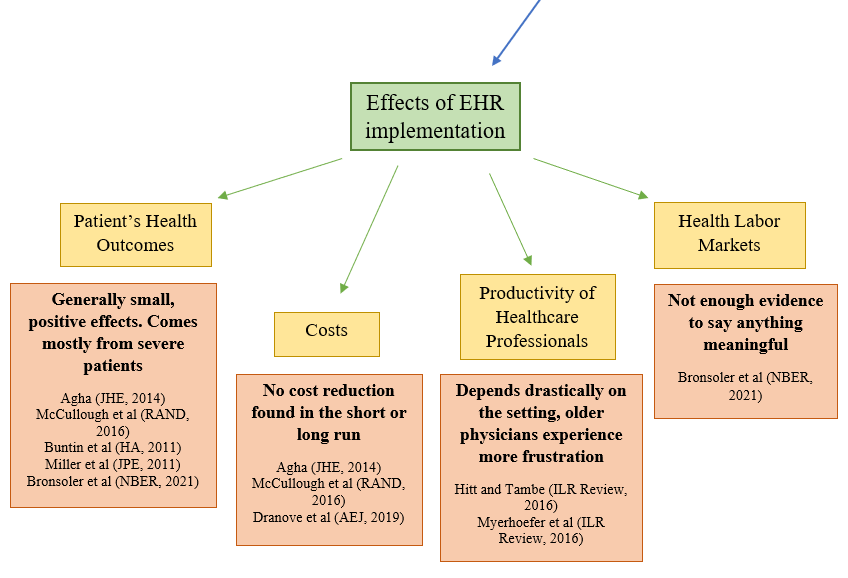
\includegraphics[scale=.45]{graphics/EHR_litgraphic.PNG}
\end{frame}


\section{Data}


\begin{frame}{Physician's Incentives}
\begin{itemize}
    \item Physician has a choice set of where to work, including multiple hospitals and office-based locations
    \item All physicians I consider work closely with at least one hospital at some point in time
    \item Some proportion of hospitals implement a new technology (an EHR)
    \item How to think about the effect on labor:
    \begin{enumerate}
        \item EHR makes seeing patients easier (or more difficult), thus the number of patients seen increases (or decreases)
        \item EHR imposes a burden with a high cost, so the physician switches to working at an office-based location where they have more control
        \item A senior physician could be tipped to retire early instead of taking on the cost of learning a new technology
    \end{enumerate}
\end{itemize}
\end{frame}


\begin{frame}{Measures of Physician Labor Market Decisions}


     Total Patients: \underline{CMS Shared Patient Data} (2009-2015)
    \begin{itemize}
        \item Sum of shared patients with all entities that have an NPI
    \end{itemize}
    
     Indicator for whether they are working
    \begin{itemize}
        \item =1 if Total Patients $>0$
    \end{itemize}
    
     Indicator for working in office-based location
    \begin{itemize}
        \item Comes from SK$\&$A database of office-based physicians
    \end{itemize}

\end{frame}

\begin{frame}{Measures of EHR Use}

Physician-level Indicator that captures exposure to \textit{any} EHR
\begin{itemize}
    \item With information on shared patients between physicians and hospitals, I limit to physicians working in hospitals
    \item Fraction of hospitals worked with that use an EHR comes from the AHA survey
    \item Similarly, I can capture hospitals that use EHRs for decision making vs. documentation using the AHA Survey IT Supplement 
\end{itemize}


\end{frame}

\begin{frame}{Other Characteristics}

Medical school graduation date, gender: \underline{Physician Compare}

\vspace{5mm}

Average size of hospital worked with (measured in beds), average hospital days operating: \underline{AHA Survey}
\end{frame}

\section{Analysis}

\begin{frame}{Event Studies}
\begin{equation*}
    Y_{it}= \sum_{t=-6}^6 \mathbbm{1}_{\{\text{relative treatment year}_{i}=t\}} + \alpha_t + \delta_{i} + \mathbb{X}_{it}
\end{equation*}
    
\end{frame}









\end{document}
